% Section: Automatic Construction of Kernel Functions
\section{Automatic Construction\\ of Kernel Functions} \label{sec:autokernel}
Choosing an appropriate \emph{Kernel Function} in a regression problem has always been a 

This section is based on the work of Duvenaud and Lloyd et. al
\cite{duvenaud2013structure,lloyd2014automatic,duvenaud2014automatic}

%% Base Kernels
\para{Base Kernels}
As we all know, different kernels can represent different kinds of data. In Figure~\ref{fig:singlekernel}, we show 4 different kinds of base kernels, each represents a specific kind of data characteristics (Table~\ref{tab:kernel}). Each function of the kernel is shown in Equation~\ref{eqa:kernel}
\begin{equation}
\left \{
\begin{aligned} \label{eqa:kernel}
k_{LIN}(x,x^{'}) &= \sigma_{b}^{2} + \sigma_{v}^{2} (x-l)(x^{'}-l) 	\\
k_{SE}(x,x^{'}) &= \sigma^2 exp(-\frac{(x-x^{'})^2}{2l^2})	\\
k_{PER}(x,x^{'}) &= \sigma^2 exp(-\frac{2sin^2 (\pi(x-x^{'})/p)}{l^2})	\\
k_{RQ}(x,x^{'}) &= \sigma^2 (1+\frac{(x-x^{'})^2}{2\alpha l^2})^{-\alpha}	\\
\end{aligned}
\right.
\end{equation}


\begin{table}[htp]
\centering
{\small
\begin{tabular}{c|c}
    \hline
    \textbf{Kernel} & \textbf{Data Characteristic} \\ 
    \hline
	   Linear(LIN) & linear functions\\
	   Squared exponential(SE) & local variation\\
	   Periodic(PER) & repeating structure\\
	   Rational quadratic(RQ) & multi-scale variation\\
	   \hline
\end{tabular}
}
\vspace{-0.1in}
\caption{Different kinds of kernels and its represented data characteristics.}
\label{tab:kernel}
% \vspace{-0.05in}
\end{table}


\begin{figure}[htp]
\begin{minipage}[htp]{1\linewidth}
	\centering
  	\subfigure[Linear(LIN)]{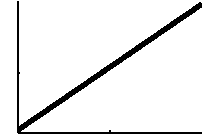
\includegraphics[width=0.48\textwidth]{figure/kernels/lin_kernel.pdf}}
	\subfigure[Squared exp(SE)]{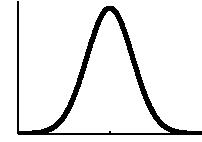
\includegraphics[width=0.48\textwidth]{figure/kernels/se_kernel.pdf}}
	\subfigure[Periodic(PER)]{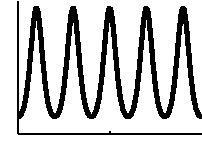
\includegraphics[width=0.48\textwidth]{figure/kernels/per_kernel.pdf}}
	\subfigure[Rational quadratic(RQ)]{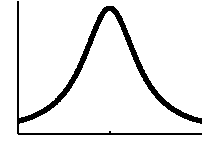
\includegraphics[width=0.48\textwidth]{figure/kernels/rq_kernel.pdf}}
% \vspace{-0.1in}
\caption{Base Kernels}
\label{fig:singlekernel} % FIG1
\end{minipage}
\vspace{-0.05in}
\end{figure}


%% Compositional Kernels
\para{Compositional Kernels}


\para{Automatic Construction}

